\section{Hadoop 2.2}
\label{sec:hadoop-2.2}

\par A partir des versions , Hadoop vient avec un nouveau composant appelé Yarn. 

\begin{figure}[h!]
  \centering
  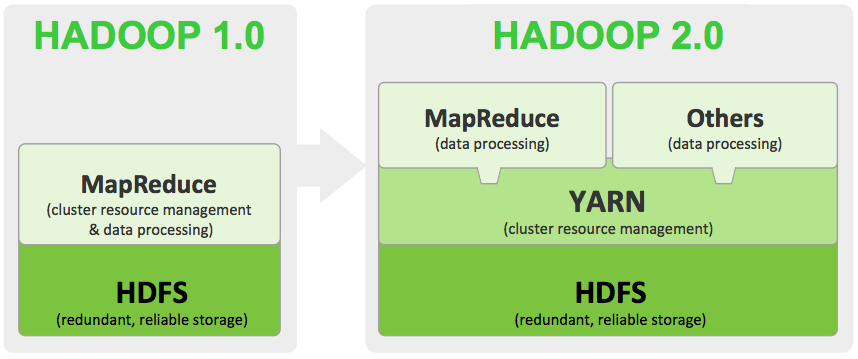
\includegraphics[width=12cm]{images/yarn.png}
  \caption{Différences entre Hadoop 1.x et Hadoop 2.x}
  \label{fig:yarn}
\end{figure}

Yarn est responsable de la gestion des ressources, et utilise des processus similaires pour leur gestion. Le NodeManager vient remplacer le TaskTracker, qui s'occupe de faire le lien entre le DataNode et le ResourceManager localisé sur le master (NameNode). Le ResourceManager déploie les applications sur les noeuds grâce à sa communication avec les NodeManagers.

--> Schéma Hadoop Yarn

\subsection{Connexion sur un ordinateur à Supélec}
\label{sec:connexion-sur-un}

\par La connexion avec un compte utilisateur précis est particulière, dans la mesure où on peut accéder à son dossier personnel, correspondant à des identifiants de connexion, depuis n'importe quelle machine. En effet, une machine est responsable de la gestion des logins, et contient les données personnelles correspondantes. Ces données transitent lors d'une connexion, ce qui peut faire croire que ces données sont présentes sur tous les ordinateurs.

\par Il est important de garder à l'esprit ce mécanisme, car c'est grâce à celui-ci que nous pourront simplifier la configuration de Hadoop sur le cluster Skynet. Malgré ces données qui ne sont pas propres à une machine, nous devons également pouvoir accéder à la mémoire de la machine physique, afin de pouvoir les utiliser comme DataNodes. Dans un premier temps, nous utiliserons le dossier \emph{/tmp} accessible en lecture écriture à n'importe qui (donc peu sécurisé, mais adapté à notre installation de test).

\begin{figure}[h!]
  \centering
  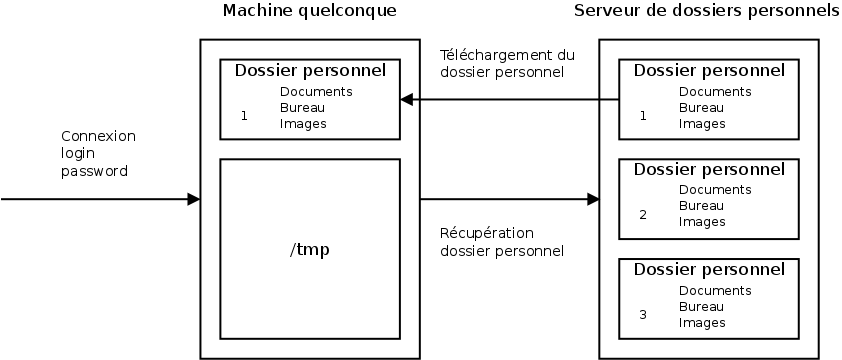
\includegraphics[width=14cm]{images/connexion_supelec.png}
  \caption{Exemple d'une connexion sur une machine quelconque}
  \label{fig:connexion_supelec}
\end{figure}

\subsection{Connexion SSH}
\label{sec:connexion-ssh}

\par Lors d'une connexion SSH, le fichier \texttt{.bash\_profile} est executé


%%% Local Variables: 
%%% mode: latex
%%% TeX-master: "CompteRendu"
%%% End: 
